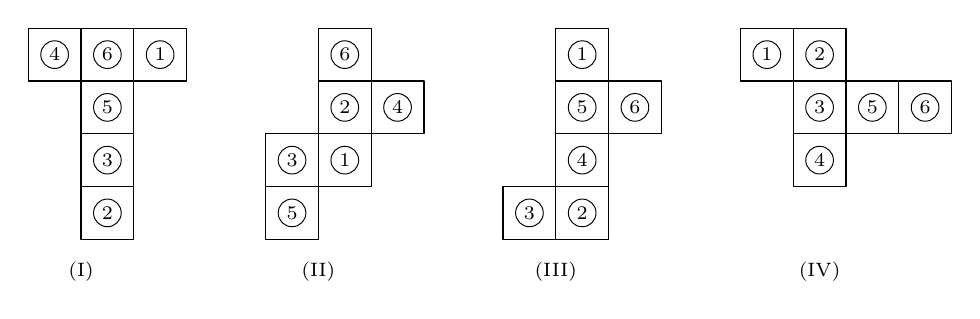
\begin{tikzpicture}[scale=.67, every node/.style={font=\scriptsize}, line cap=round, line join=round]
  \tikzset{face/.style={draw=black, line width=.42pt}, circled/.style={draw=black, circle, line width=.35pt, minimum size=10pt, inner sep=.15pt}}

  % (I)
  \begin{scope}
    \foreach \x/\y/\n in {-1/3/4,0/3/6,1/3/1,0/2/5,0/1/3,0/0/2} {
      \draw[face] (\x,\y) rectangle ++(1,1);
      \node[circled] at (\x+.5,\y+.5) {\n};
    }
    \node[below] at (0,-.25) {(I)};
  \end{scope}

  % (II)
  \begin{scope}[xshift=4.5cm]
    \foreach \x/\y/\n in {0/3/6,0/2/2,1/2/4,-1/1/3,0/1/1,-1/0/5} {
      \draw[face] (\x,\y) rectangle ++(1,1);
      \node[circled] at (\x+.5,\y+.5) {\n};
    }
    \node[below] at (0,-.25) {(II)};
  \end{scope}

  % (III)
  \begin{scope}[xshift=9cm]
    \foreach \x/\y/\n in {0/3/1,0/2/5,1/2/6,0/1/4,-1/0/3,0/0/2} {
      \draw[face] (\x,\y) rectangle ++(1,1);
      \node[circled] at (\x+.5,\y+.5) {\n};
    }
    \node[below] at (0,-.25) {(III)};
  \end{scope}

  % (IV)
  \begin{scope}[xshift=13.5cm]
    \foreach \x/\y/\n in {-1/3/1,0/3/2,0/2/3,1/2/5,2/2/6,0/1/4} {
      \draw[face] (\x,\y) rectangle ++(1,1);
      \node[circled] at (\x+.5,\y+.5) {\n};
    }
    \node[below] at (.5,-.25) {(IV)};
  \end{scope}
\end{tikzpicture}
